%% ****** Packages needed for LaTeX document: ****** 
%%\usepackage{graphicx} %%\postscript includes
%%\usepackage{multirow} %%\multirow command
%%\usepackage{wasysym} %%\permil command
%%\usepackage{gensymb} %%\degree command
\begin{table}
\begin{center}
\begin{tabular}{|c|}
\hline
\begin{large} CircSection 1 \end{large}\\
\hline
Text describing the role/position of the section in the structure.\\
\hline
\begin{tabular}{c|l}
\begin{minipage}{85mm}
\vspace{2mm}
\begin{center}
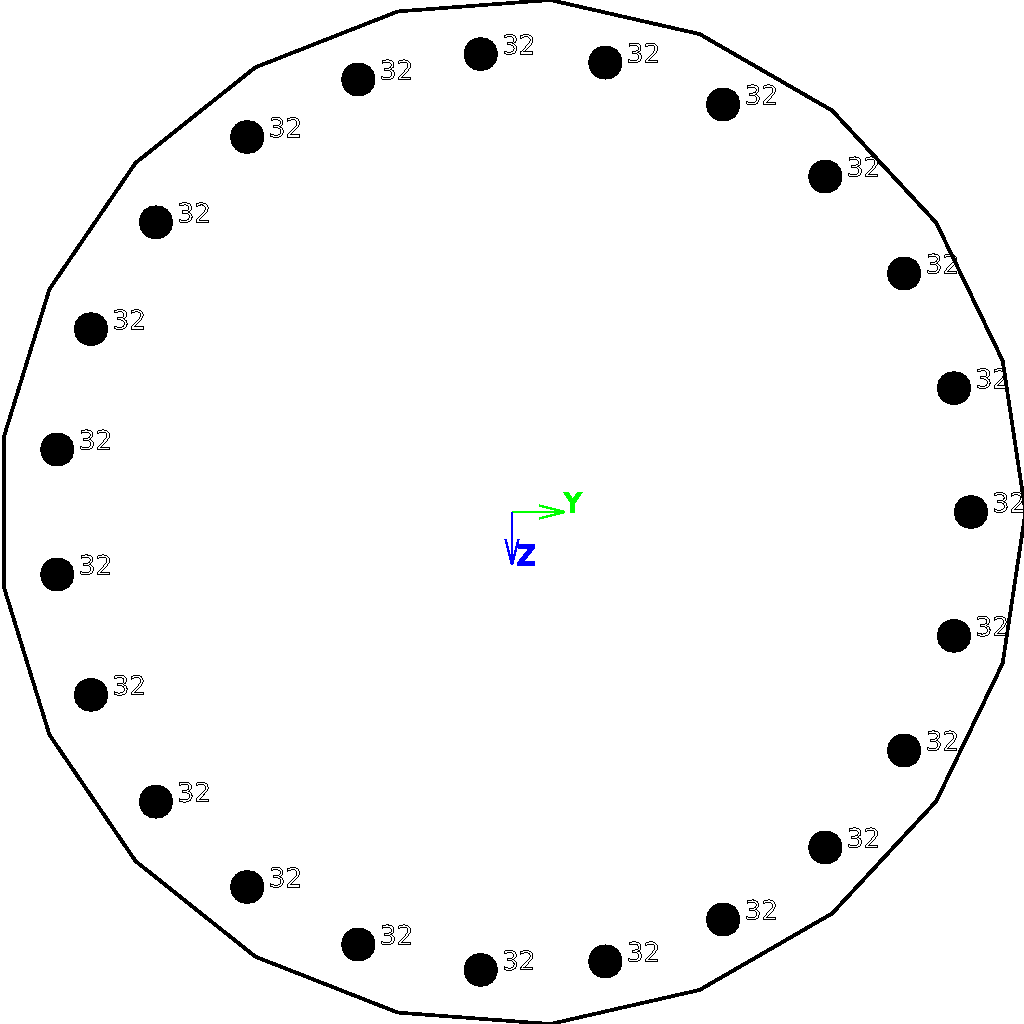
\includegraphics[width=70mm]{CircSection1}
\end{center}
\vspace{1pt}
\end{minipage} & 
\begin{tabular}{l}
ext. radius: \\
$r_{ext}= 0.50\ m$\\
int. radius: \\
$r_{int}= 0.00\ m$\\
\end{tabular} \\
\end{tabular} \\
\hline
\textbf{Materials - mechanical properties}:\\
\hline
\begin{tabular}{ll}
Concrete: HA30 & Modulus of elasticity: $E_c= 28.58\ GPa$\\
\hline
Steel: B500S & Modulus of elasticity: $E_s= 200.00\ GPa$\\
\end{tabular} \\
\hline
\textbf{Sections - geometric and mechanical characteristics}:\\
\hline
Gross section:\\
\hline
\begin{tabular}{ll}
$A_{gross}= 0.774\ m^2$ & \multirow{3}{*}{Inertia tensor ($cm^4$): $ \left( \begin{array}{ccc}981.75 & 0.00 & 0.00 \\ 0.00 & 476.42 &  0.00 \\ 0.00 &  0.00 & 476.42 \end{array} \right)$} \\
& \\
C.O.G.: $(0.000,0.000)\ m$  & \\
\end{tabular} \\
\hline
Homogenized section:\\
\hline
\begin{tabular}{ll}
$A_{homog.}= 0.967\ m^2$ & \multirow{3}{*}{Inertia tensor ($cm^4$): $ \left( \begin{array}{ccc}981.75 & 0.00 & 0.00 \\ 0.00 & 661.35 &  0.00 \\ 0.00 &  0.00 & 677.28 \end{array} \right)$} \\
& \\
C.O.G.: $(0.004,0.000)\ m$  & \\
\end{tabular} \\
\hline
\textbf{Passive reinforcement}:\\
\hline
\begin{tabular}{ll}
Total area $A_s=193.02\ cm^2$ & Geometric quantity $\rho= 24.95\permil$\\
\end{tabular} \\
\hline
Layers of main reinforcement:\\
\hline
\begin{tabular}{cccccccc}
Id & N$^o$ bars & $\phi$ & area & c. geom. & eff. cover & $y_{COG}$ & $z_{COG}$\\
 &  & $(mm)$ & $(cm^2)$ & $(\permil)$ & $(cm)$ & $(m)$ & $(m)$\\
\hline
 & 24 & 32 &  8.04 & 1.04 &  4.7 & 0.019 & -0.000\\
\end{tabular} \\
\hline
Layers of shear reinforcement:\\
\hline
\begin{tabular}{cccccccc}
Id & N$^o$ branch & $\phi$ & area & spac. & area/m & $\alpha$ & $\beta$\\
 &  & $(mm)$ & $(cm^2)$ & $(cm)$ & $(cm^2/m)$ & $( \degree)$ & $( \degree)$\\
\hline
 & 4 & 12 & 18.10 & 25.0 & 72.38 & 90.0 & 45.0\\
\end{tabular} \\
\hline
\end{tabular}
\end{center}
\caption{Text describing the role/position of the section in the structure. (CircSection 1).} \label{tb_CircSection_1}
\end{table}
